\newpage
\null
\thispagestyle{empty}
\newpage
\section{Experimenty}
%TODO upravit
\label{experiments}
V priebehu práce bolo nutné experimentovať v naozaj veľkom množstve s najrôznejším počtom vecí od typov neurónových sietí, datasetov až po rôzne prístupy k riešeniu zadaného problému.

Prvotné experimenty vykonávané vrámci predmetu Počítačové videnie\footnote{http://vgg.fiit.stuba.sk/teaching/computer-vision/} sú zachytené v kapitole \ref{first_experiments}. Ďalšie experimenty potom prebiehali postupne s konvolučnou neurónovou sieťou (kapitola \ref{experiments_cnn}), konvolučným autoenkóderom (kapitola \ref{experiments_autoencoder}) a autoenkóderom s predtrénovanou sieťou VGG-Net (kapitola \ref{experiments_vgg_net}). Pri každom modeli sme odskúšali nespočetné množstvo rôznych konfigurácií, pre popis sme ale vybrali len tie s najlepšími výsledkami pre jednotlivé časti. 

\subsection{Implementačné prostredie}

Všetky nižšie popisované experimenty boli naimplementované v jazyku Python za použitia najrôznejších knižníc, hlavne pre prácu s obrázkami a neurónovými sieťami (bližšie popísané v prílohe \ref{technical_doc}). Najdôležitejšími knižnicami sú:
\begin{itemize}
	\item TensorFlow\footnote{https://www.tensorflow.org/} - open-source knižnica pre prácu s neurónovými sieťami a strojovým učením
	\item Keras\footnote{https://keras.io/} - vysoko úrovňová knižnica pre prácu s neurónovými sieťami, beží na nižšie úrovňovými knižnicami ako Theano či TensorFlow
	\item Matplotlib\footnote{https://matplotlib.org/} - knižnica pre 2D vykresľovanie v Python-e
	\item OpenCV\footnote{https://opencv.org/, https://pypi.org/project/opencv-python/} - open-source knižnica pre počítačové videnie a strojové učenie
	
	Trénovanie modelov v experimentoch prebiehalo na GPU.
\end{itemize}

\subsection{Prvotné experimenty}
\label{first_experiments}
Pre prvotné experimenty sme sa rozhodli zvoliť problém predikcie vizuálnej pozornosti v častiach obrázkov, konkrétne v tzv. regiónoch záujmu (z angl. regions of interest, ROIs), ktoré sme zvolili v okolí fixácií na obrázky.

\subsubsection{Úprava datasetu}
\label{dataset}

V tejto fáze prvotných experimentov sme pracovali s datasetom zloženým z niekoľkých voľne dostupných dataset-ov vizuálnej pozornosti (CAT2000\cite{borji2015cat2000}, NUSEF\footnote{http://mmas.comp.nus.edu.sg/NUSEF.html}, ...).
Keďže vo viacerých z nich chýbali úplné informácie k výpočtu máp výraznosti, rozhodli sme sa ich získať z dostupných obrázkov máp výraznosti, kedy sme ich načítali ako jednofarebný  obrázok v odtieňoch sivej (z angl. grayscale) - hodnota pixelu vtedy prakticky reprezentuje intenzitu. Ďalej sme spolu pre vstupné obrázky a mapy výraznosti extrahovali regióny záujmu, ktoré sme zvolili v okolí fixácií - vizualizácia popisovanej extrakcie je zobrazená na obrázku \ref{roi_image}. Nevyhovujúce časti datasetov (ako napr. abstraktné umienie, fraktály, cartoon obrázky, ...) boli odfiltrované.

\begin{figure}[H]
	\begin{center}
		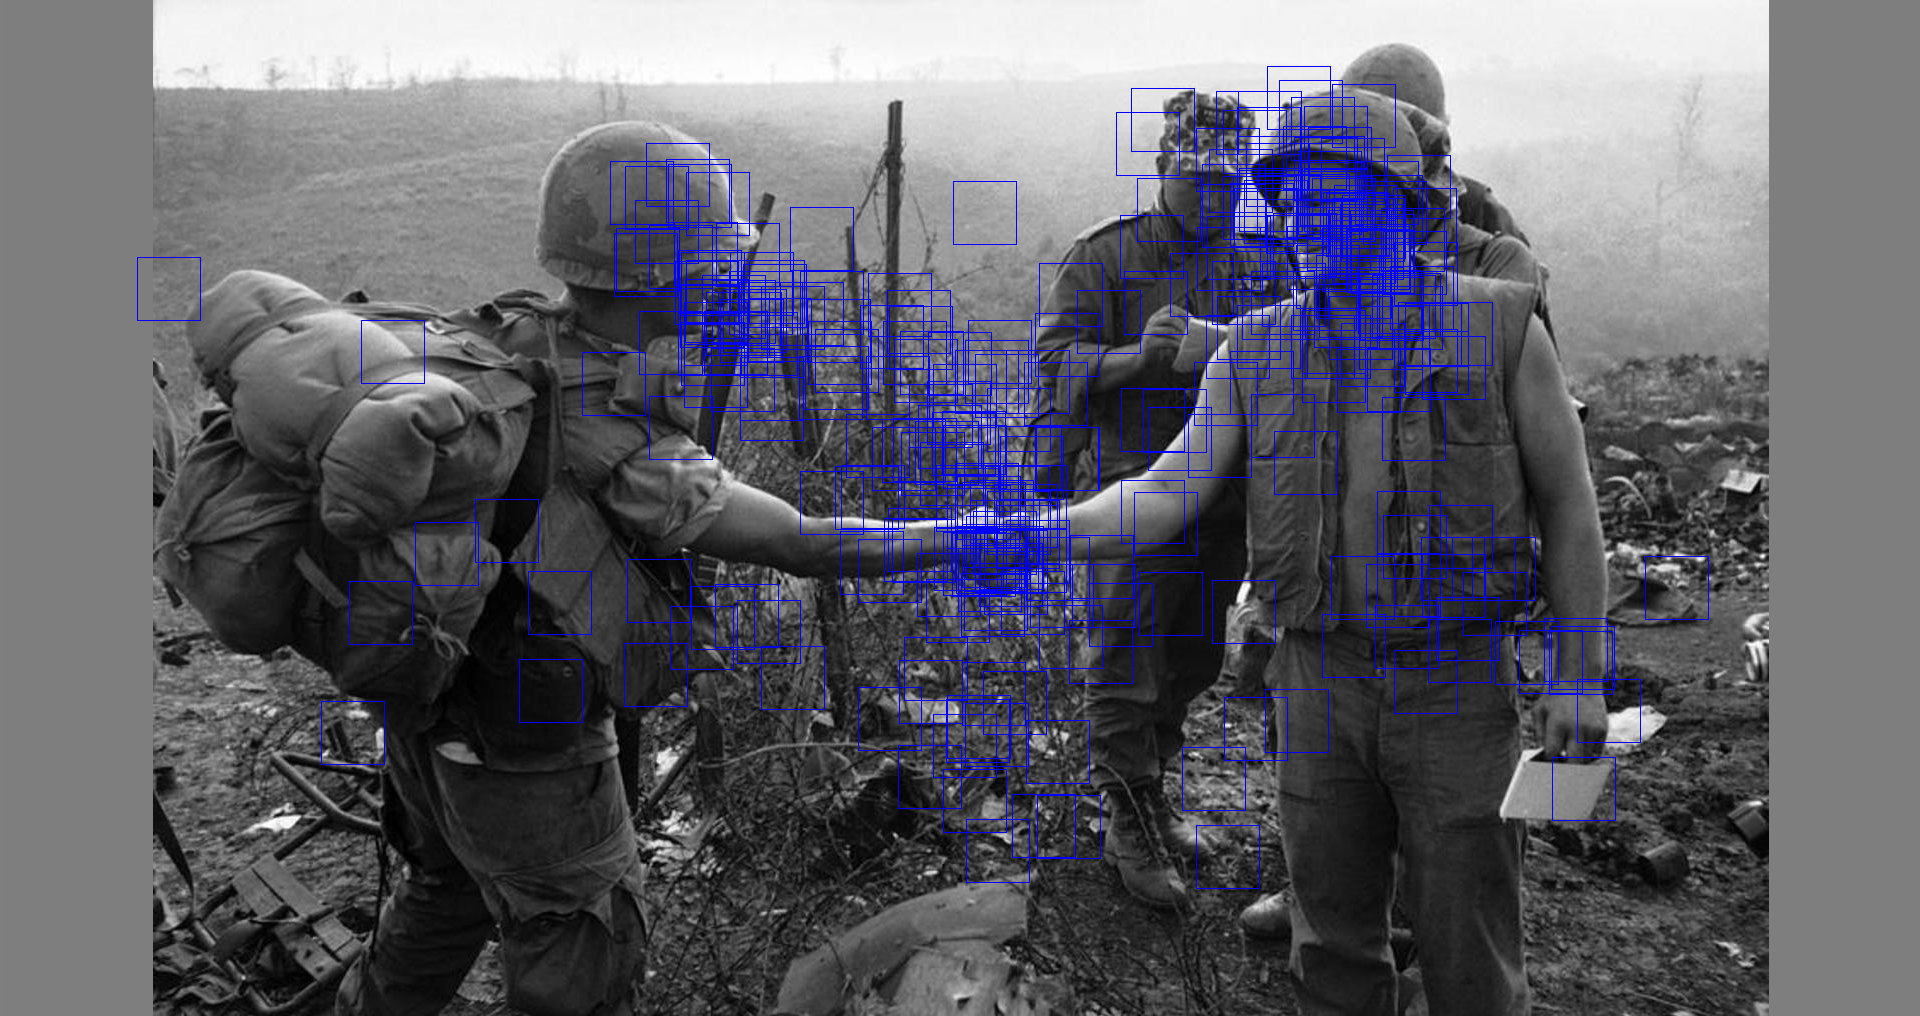
\includegraphics[scale=0.13]{img.PNG}
		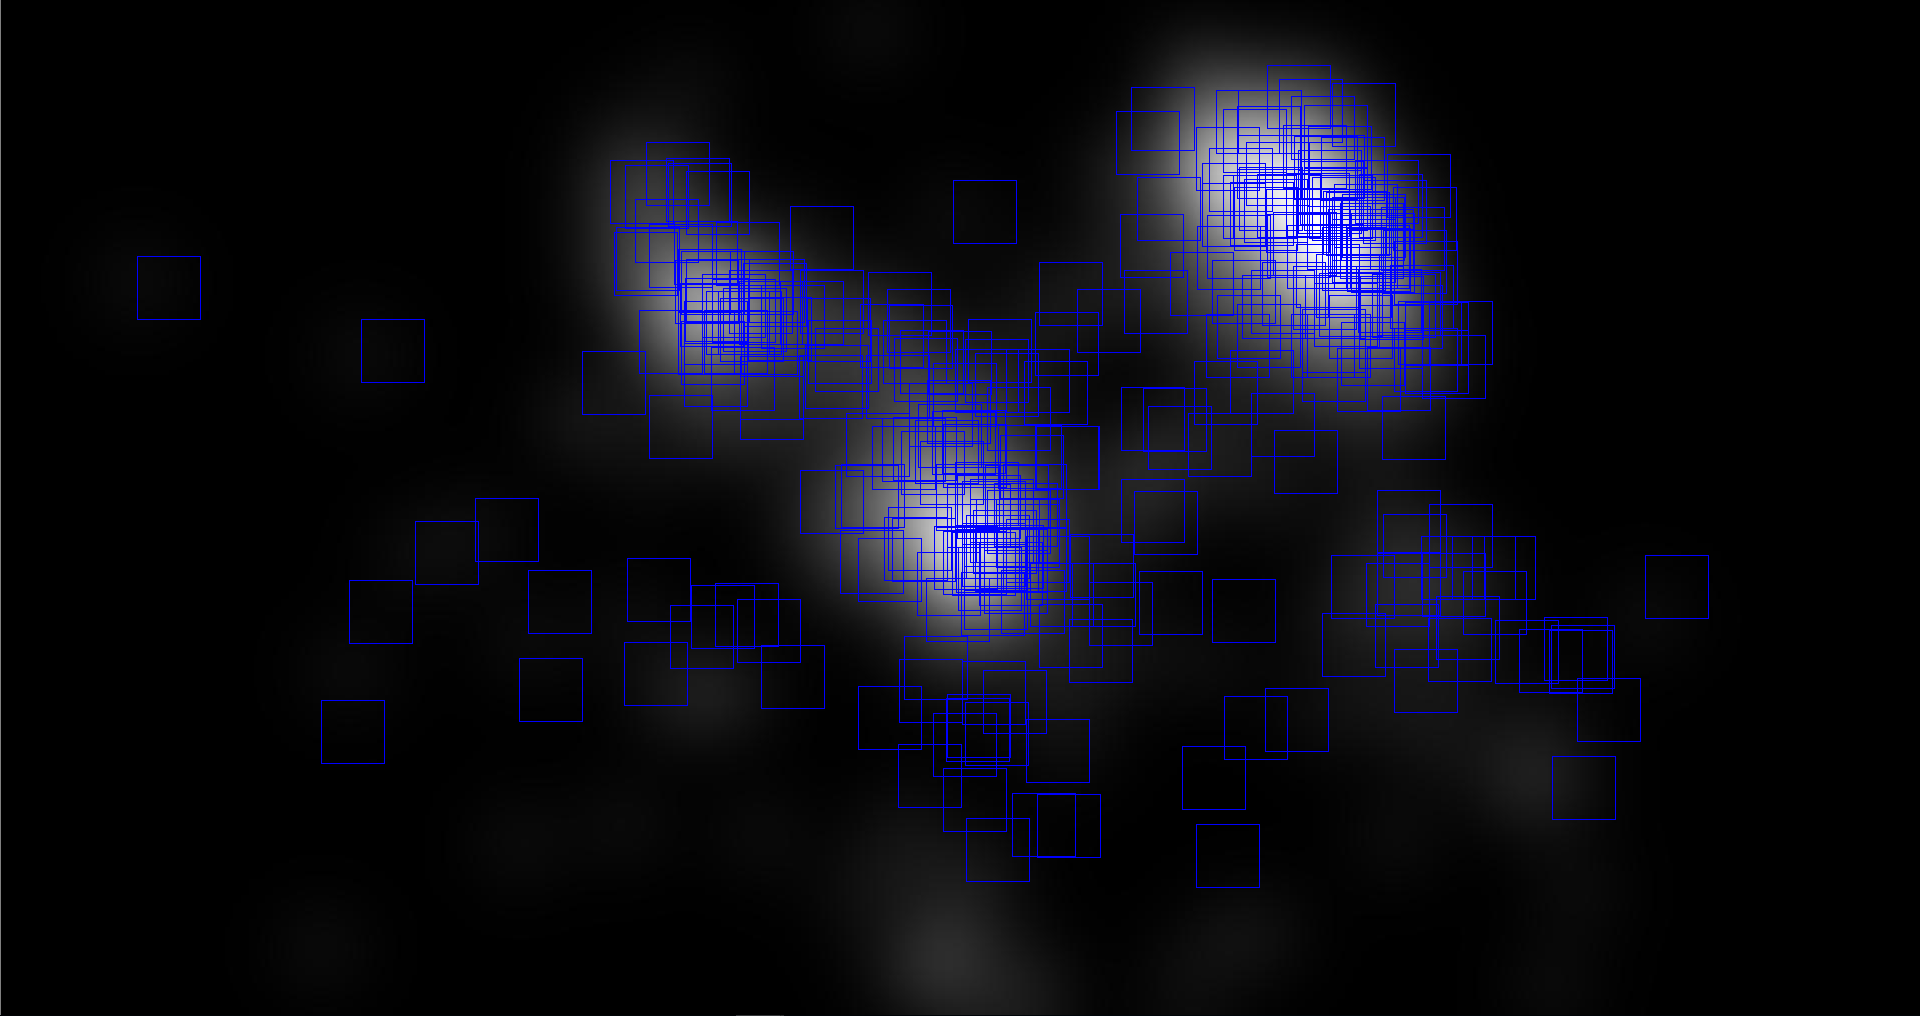
\includegraphics[scale=0.13]{map.PNG}
		\caption[Vizualizácia extrakcie regiónov záujmu]{
			Vizualizácia extrakcie regiónov záujmu, vľavo obrázok, vpravo mapa výraznosti k nemu
		}\label{roi_image}
	\end{center}
\end{figure}

Takto získané dáta boli ďalej pre neurónovú sieť normalizované, dokopy sme si nakoniec zaistili zhruba 500 000 vzoriek.
\newline

\subsubsection{Výsledky}

Navrhovanú konvolučnú neurónovú sieť (kapitola \ref{nn_popis}) sme trénovali na priravenom datasete, ktorý bol rozdelený štandardne v pomere 80:10:10 (80 - trénovanie, 10 - validácia, 10 - testovanie). Validácia prebiehala po každej iterácii a trénovanie končilo v momente keď sa chyba na validačných dátach začala výrazne odlišovať oproti najnižšej dosiahnutej (pomaly dochádzalo k pretrénovaniu). V závere mala sieť chybu predikcie na testovacích dátach na úrovni \textit{0.29}, chyba bola počítaná ako priemer chýb v každom bode obrázka. Na obrázku \ref{results_image} možno vidieť porovanie predikovaných máp výraznosti s originálnymi a so vstupnými obrázkami. 

\begin{figure}[H]
	\begin{center}
		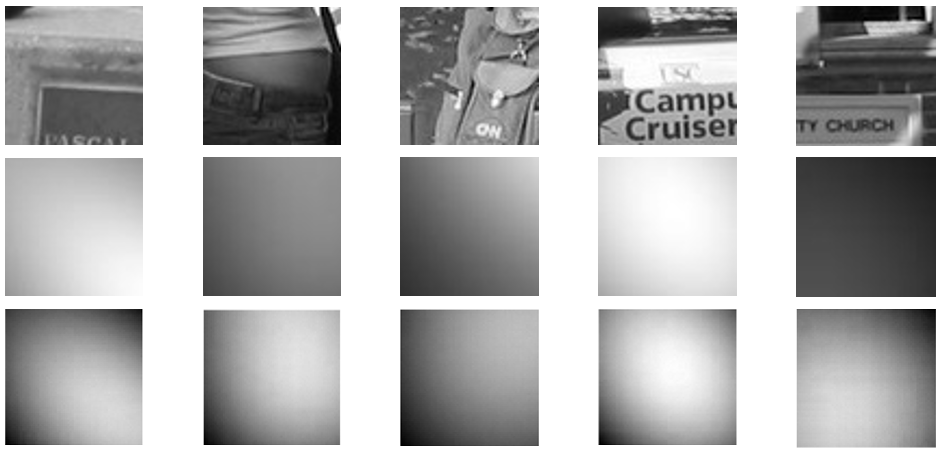
\includegraphics[scale=0.5]{predicted_saliency.PNG}
		\caption[Porovnanie prvotných výsledkov]{
			Porovnanie predikcií (dolu) s originálnymi mapami výraznosti (v strede) voči vstupným obrázkom (hore)
		}\label{results_image}
	\end{center}
\end{figure}

Pri snahe vypočítať metriky pre predikcie sme narazili na problém, ktorý sme si na začiatku neuvedomili. Väčšina metrík evaluuje mapu výraznosti voči binárnej matici reprezentujúcej fixácie na obrázok. Vzhľadom na to, že našim vstupom boli regióny záujmy v okolí fixácií, vo väčšine prípadov tieto binárne matice obsahovali len jednu fixáciu. Vďaka tomu mali metriky (AUC, sAUC, NSS) nezmyselne vysoké hodnoty. Z tohto dôvodu ich teda považujeme za nerelevantné a jediná metrika, podľa ktorej sa môžeme riadiť, je korelačný koeficient, keďže ten evaluuje predikovanú mapu voči tej pôvodnej. Jeho hodnoty na testovacích dátach sa v priemere pohybovali na hranici 0.563.

\subsection{Konvolučná neurónová sieť}
\label{experiments_cnn}

Ďalším experimentom bolo použitie klasickej konvolučnej neurónovej siete rovnako ako v predchádzajúcom prípade, tentokrát ale na celých obrázkoch. Ako dataset bol použitý spracovaný DUT-OMRON dataset (popísaný v kapitole \ref{dataset_description}) rozdelený podobne v pomere 80:10:10 (80 - trénovanie, 10 - validácia, 10 - testovanie), validácia bola tiež po každej epoche, trénovanie ale končilo v momente keď validačná chyba začala stúpať. Na obrázku nižšie možno vidieť vývoj jednotlivých chýb počas trénovania. Chyba bola počítaná ako priemier chýb predikcií v jednotlivých bodoch obrázka.

\begin{figure}[H]
	\begin{center}
	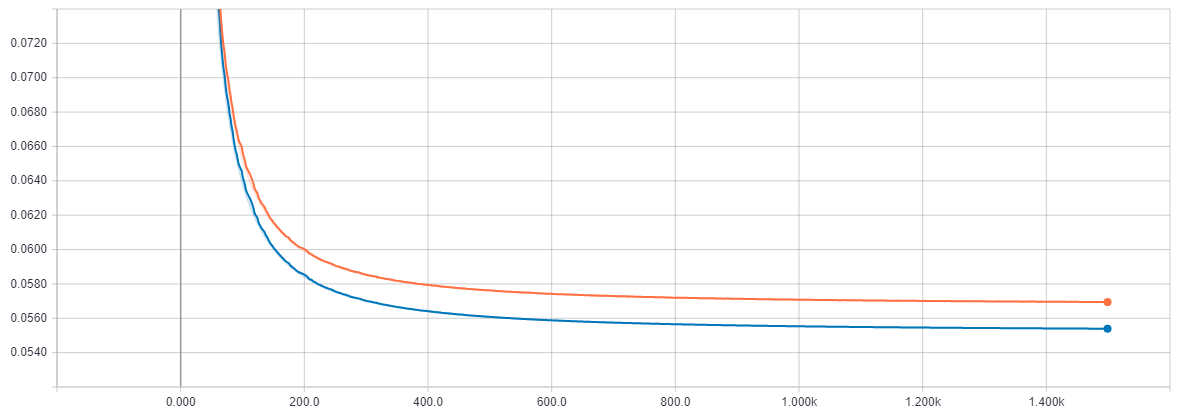
\includegraphics[scale=0.3]{nn_loss_no_outliers.png}
		\caption[Vývoj chyby počas trénovania konvolučnej neurónovej siete]{
			Graf zobrazujúci vývoj chyby neurónovej siete po odstránení extrémov počas 300 epoch - modrá farba reprezentuje chybu na trénovacích dátach, oranžová chybu na validačných dátach
		}\label{cnn_loss_outliers}
	\end{center}
\end{figure}

Z vyššie uvedených grafov vyplýva, že sieť bola schopná najvýraznejšie znížiť chybu predikcií behom prvých 50 epoch. Z jej počiatočnej hodnoty približne \textit{0.6709} klesla až na \textit{0.1321} na trénovacích dátach, na validačných dosahovala hodnotu \textit{0.1396}. Pri finálnom testovaní bola priemerná chyba približne \textit{0.1459}. Na prvý pohľad sa to môže javiť ako solídny výsledok, po vizualizovaní predikcií sme ale zistili, že sieť sa prakticky naučila predikovať ako najvýraznejšiu časť obrázka vždy len jeho stred, príklad predikcie je na obrázku \ref{cnn_results}.

\begin{figure}[H]
	\begin{center}
		
		%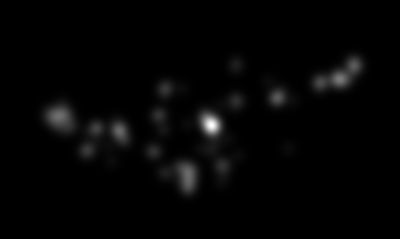
\includegraphics[width=10.58cm,height=6.32cm]{cnn_plane_heatmap.png}
		%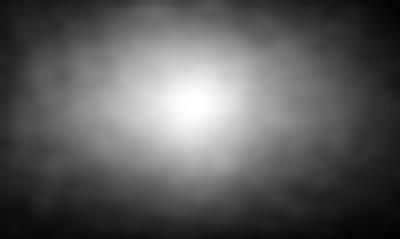
\includegraphics[width=10.58cm,height=6.32cm]{cnn_plane_predict.png}
		%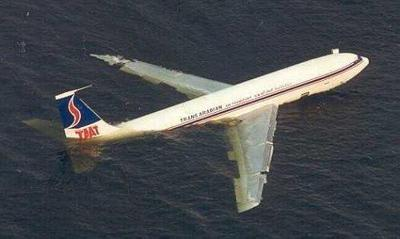
\includegraphics[width=10.58cm,height=6.32cm]{cnn_plane.png}
		%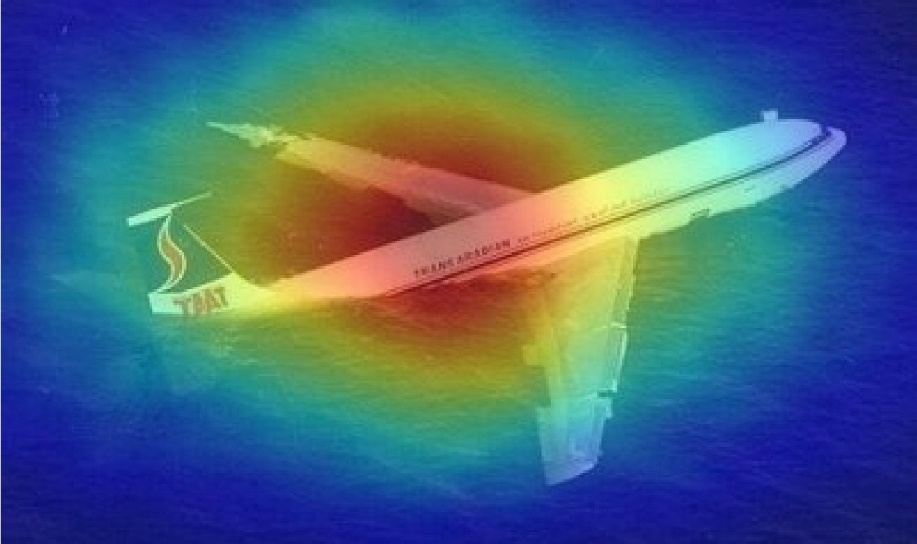
\includegraphics[width=10.58cm,height=6.32cm]{cnn_predict_on_plane.png}
		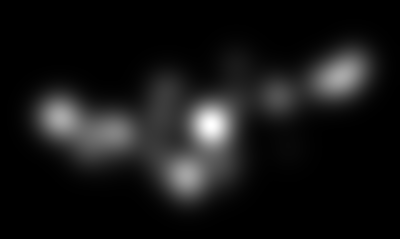
\includegraphics[scale=0.4]{cnn_plane_heatmap_regenerated.png}
		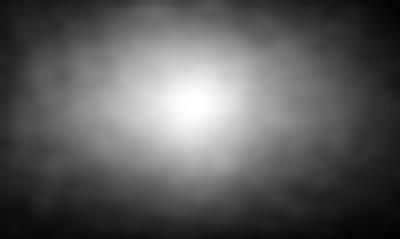
\includegraphics[scale=0.4]{cnn_plane_predict.png}
		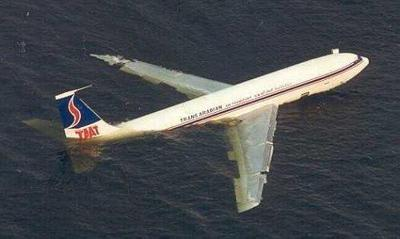
\includegraphics[scale=0.4]{cnn_plane.png}
		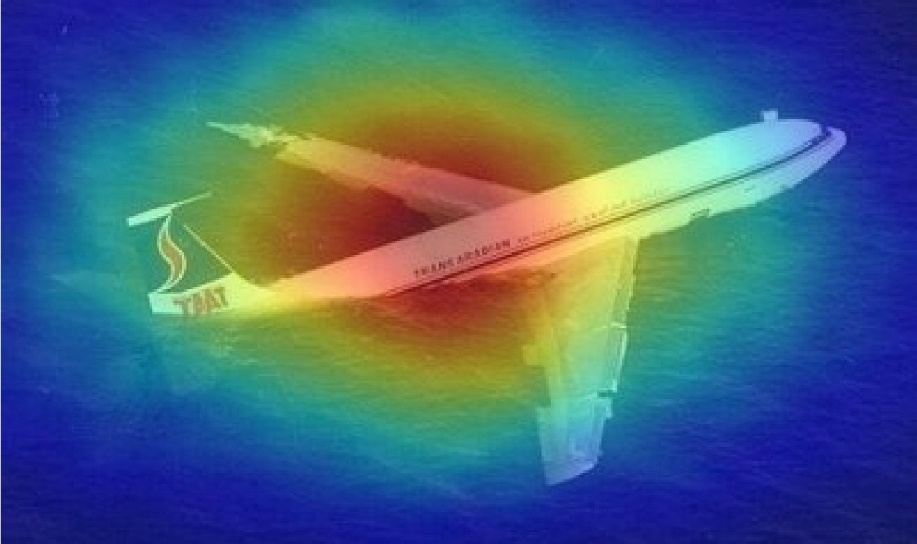
\includegraphics[scale=0.534]{cnn_predict_on_plane.png}
		\caption[Vzorka predikcie konvolučnej neurónovej siete]{
			Vľavo hore originálna mapa vizuálanej pozornosti, vpravo hore predikovaná mapa, vľavo dole obrázok pre prislúchajúce mapy výraznosti, vpravo dole zobrazenie predikcie na obrázku
		}\label{cnn_results}
	\end{center}
\end{figure}

Vyššie zobrazené správanie môže byť spôsobené napríklad relatívne malou veľkosťou vstupných obrázkov, kvôli veľkej pamäťovej náročnosti siete. 

\subsection{Konvolučný autoenkóder}
\label{experiments_autoencoder}

Ďalšou architektúrou, ktorú sme sa rozhodli vyskúšať, bol konvolučný autoenkóder (navrhnutý v kapitole \ref{autoencoder_design}). Použitý dataset a jeho rozdelenie bolo rovnaké ako v predošlom experimente, trénovanie ale končilo až keď validačná chyba za posledných \textit{n} epoch neklesla. Ako funkcia chyby bola použitá priemerná absolútna chyba (z angl. mean absolute error, MAE), ktorá meria rozdiel medzi dvomi spojitými premennými, v našom prípade medzi reálnou a predikovanou mapou výraznosti, resp. ich pixelmi. Priebeh učenia možno vidieť na obrázku \ref{autoencoder_loss}. 

\begin{figure}[H]
	\begin{center}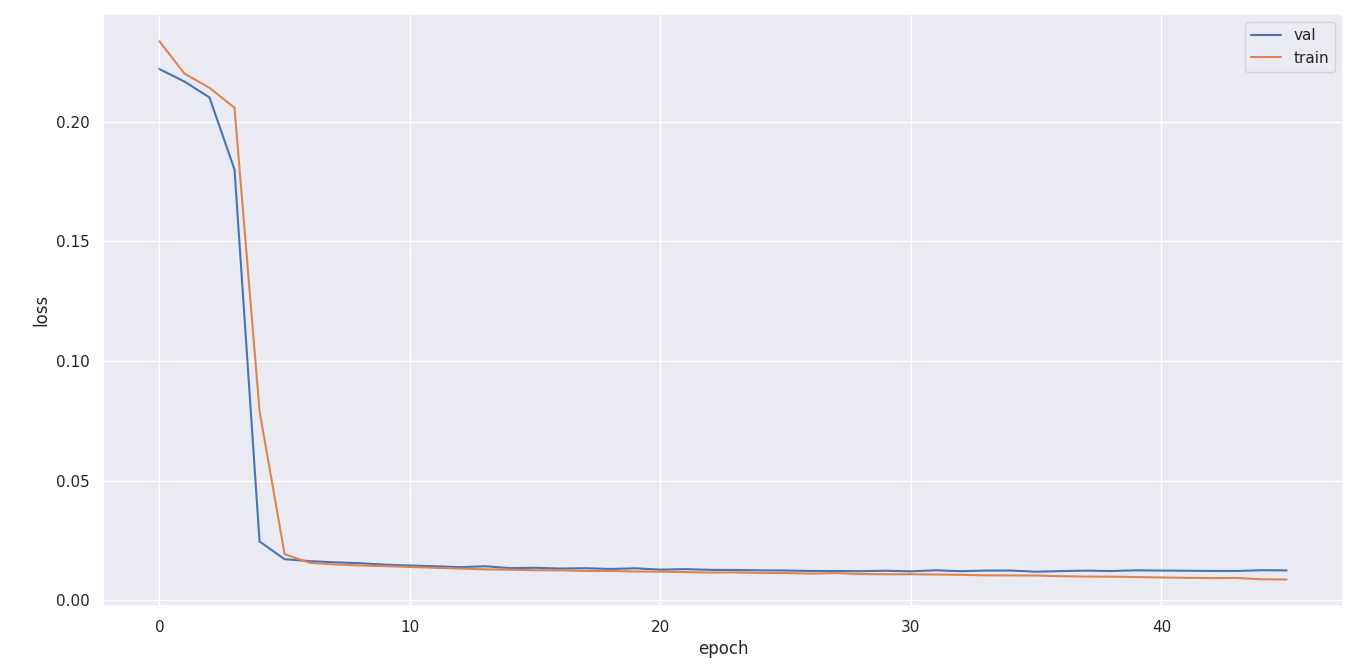
\includegraphics[scale=0.2]{autoencoder_loss.png}
		\caption[Vývoj chyby počas trénovania autoenkóderu]{
			Vývoj chyby počas trénovania, oranžovaná reprezentuje trénovaciu, modrá validačnú 
		}\label{autoencoder_loss}
	\end{center}
\end{figure}

Z obrázku je vidieť, že učenie prebiehalo počas 45 epoch, chyba najvýraznejšie klesla počas prvých šiestich epoch. Z počiatočnej hodnoty \textit{0.2336} (trénovacie dáta) a \textit{0.2219} (validačné dáta) bola schopná klesnúť až na hodnotu \textit{0.00874} (trénovacie dáta) a \textit{0.01245} (validačné dáta). Priemerná hodnota chyby pri testovaní na dátach, ktoré sieť nikdy nevidela, bola na úrovni \textit{0.01301}. Vizualizácie porovnanie predikcií sú zobrazené na obrázku \ref{autoencoder_results}.

\begin{figure}[H]
	\begin{center}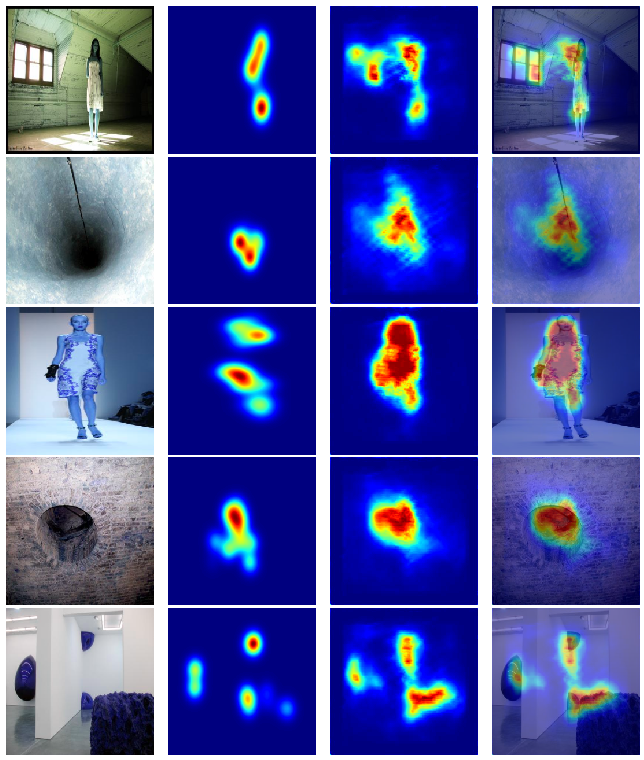
\includegraphics[scale=0.6]{autoencoder_results.png}
		\caption[Porovnanie predikcií autoenkóderu voči reálnym mapám výraznosti]{
			Porovnanie predikcií autoenkóderu, zľava vstupný obrázok, potom originálna mapa výraznosti, predikovaná mapa výraznosti a nakoniec predikcia zobrazená na obrázku. 
		}\label{autoencoder_results}
	\end{center}
\end{figure}

Z vyššie uvedených vizualizácií jasne vidieť, že sieť bola schopná naučiť sa isté výrazné súvislosti z dát, predikcie však nie sú úplne presné. Na rozdiel od siete z predošlého experimentu už nepredikuje všetko do stredu, ale je schopná označiť aj viacero výrazných objektov. To môže byť spôsobené napríklad väčšou veľkosťou vstupných obrázkov. Nakoľko autoenkóder si interne vstupné dáta zkomprimuje a zníži ich dimezionalitu, je v porovnaní zo spomínanou sieťou z predchádzajúceho experimentu pri rovnako veľkých vstupných obrázkoch menej pamäťovo náročný.

Zaujímavým javom, ktorý sme si všimli pri experimentovaní s týmto typom siete je, že hodnota chyby predikcie siete pri našom probléme nie je úplne smerodajná informácia. Pri použití napr. priemernej štvorcovej chyby (z angl. mean square error, MSE) bola výsledná chyba \textit{0.0000431}, ale predikcie boli v podstate len prázdne mapy bez akýchkoľvek výrazných častí. Tiež pri použití ešte väčšieho množstva konvolučných vrstiev sa použitá priemerná absolútna chyba zmenšila počas trénovania viac, avšak sieť sa v tomto prípade naučila predikovať najviac výrazné časti obrázkov vždy len do stredu, podobne ako pri konvolučnej neurónovej sieti z predošlého experimentu. Práve preto sme kvalitu modelov a predikcií vyhodnocovali metrikami vizuálnej pozornosti (kapitola \ref{metric}), ktorých prehľadné porovnanie aj so závermi je uvedené v \ref{results}.

\subsection{Autoenkóder s predtrénovaným modelom VGG16}
\label{experiments_vgg_net}

Pre tento experiment sme si vybrali sieť od A. Meyer-a\footnote{https://github.com/arthurmeyer/Saliency\_Detection\_Convolutional\_Autoencoder} popisovanú v kapitole \ref{object_detection}, ktorá je voľne dostupná. Jedná sa o variáciu autoenkóderu využívajúceho sieť VGG16 k predikcii binárnej mapy zobrazujúcej dominantné objekty v scéne. Pôvodná hypotéza bola, že vďaka použitému predtrénovanému modelu VGG16 pre detekciu objektov bude sieť lepšie rozumieť vstupný obrázkom a preto pri dodatočnom dotrénovaní k predikcii máp vizuálnej pozornosti bude dávať lepšie výsledky. Po menších úpravách siete sme pristúpili k trénovaniu na našom datasete, postupný vývoj chyby počas trénovania možno vidieť na obrázku \ref{vgg_pretrained_loss}. Validácia prebiehala každých 100 epoch, trénovanie končilo v momente keď minimálna hodnota chyby za posledných \textit{n} epoch neklesla. 
 
\begin{figure}[H]
	\begin{center}
		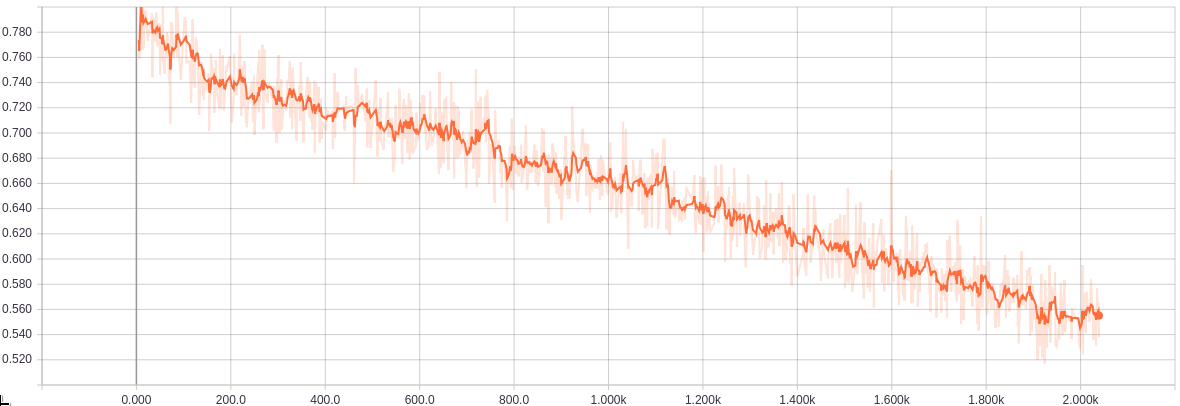
\includegraphics[scale=0.3]{vgg_pretrained.png}
		\caption[Vývoj chyby počas trénovanie siete s predtrénovaným modelom VGG16]{
			Graf zobrazujúci vývoj chyby po odstránení extrémov pri použití predtrénovaného modelu VGG16 
		}\label{vgg_pretrained_loss}
	\end{center}
\end{figure}

Na prvý pohľad sa môže zdať, že sieť sa bola schopná naučiť aspoň nejaké závislosti z dát. Po vizualizovaní dát sme ale zistili, že sme sa veľmi mýlili a snaha o dotrénovanie nepriniesla žiadne ovocie. Vizualizované výsledné dáta, ktoré mali reprezentovať mapy výraznosti, rozhodne ako mapy výraznosti nevyzerali a sieť sa nenaučila nič užitočné. Výsledkom boli len úplne náhodné hodnoty, ktoré sa ani zďaleko neblížili realite. Preto možno považovať tento experiment za nepríjemnú slepú uličku.

\subsection{Kombinácia autoenkóderu s VGG16 sieťou}

V jednom z experimentov sme testovali architektúru inšpirovanú riešením  zachytávajúcim sémantickú medzeru pri predikcii vizuálnej pozornosti (kapitola \ref{semantic_gap}). Prakticky podľa návrhu v kapitole \ref{vgg16_combination_with_autoencoder} sme zostrojili neurónovú sieť kombinujúcu detekciu objektov pomocou predtrénovanej siete VGG16 a predikciu vizuálnej pozornosti pomocou autoenkóderu. 

Sieť sme potom postupne trénovali v 2 dvoch konfiguráciach:
\begin{itemize}
	\item s vypnutím učenia pre vrstvy VGG16 siete - išlo nám o snahu zachovať kontext detekcie objektov.
	\item so zapnutím učenia pre vrstvy VGG16 siete - po odskúšaní vyššie uvedenej konfigurácie sme zistili, že mapy vizuálnej pozornosti nemajú až tak vysokú mieru granularity a chceli sme to zmeniť dotrénovaním vrstiev pre detekciu objektov. 
\end{itemize}

Na obrázku \ref{vgg16_loss_trainable_vs_nontrainable} je zobrazený vývoj  trénovacej a validačnej chyby počas učenia. Ako chyba bola zvolená binárna krížová entropia (z angl. binary cross entropy) v kombinácii s adadelta optimizérom a algoritmom spätného šírenia chyby. Učenie končilo v momente, keď sa za posledných \textit{n} epoch nezlepšila validačná chyba.

\begin{figure}[H]
	\begin{center}
		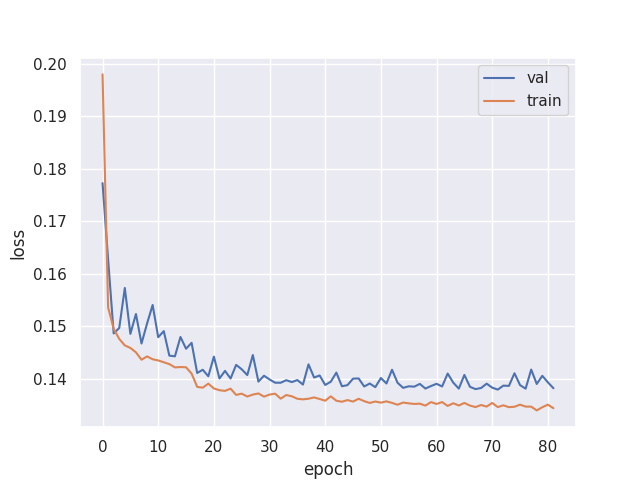
\includegraphics[scale=0.415]{vgg16_nontrainable_loss.png}
		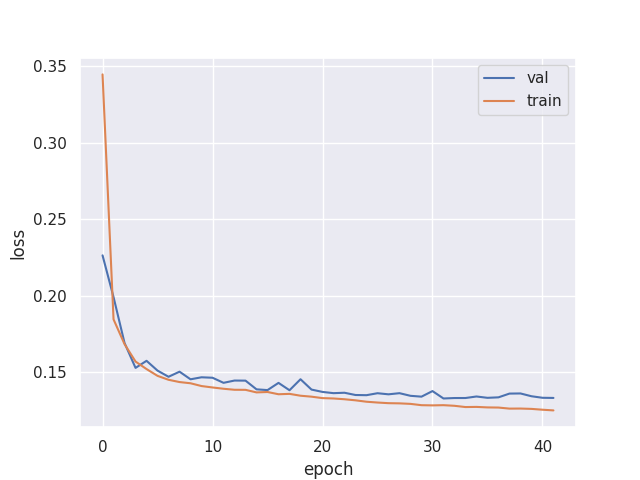
\includegraphics[scale=0.415]{vgg16_trainable_loss.png}
		\caption[Porovnanie vývoja chyby predikcie počas trénovania kombinácie autoenkóderu s VGG16 sieťou]{
			Porovnanie vývoja chyby počas trénovania, oranžová reprezentuje chybu na trénovacích dátach, modrá na validačných. Vľavo graf pre vypnuté učenie na vrstvách detekcie objektov, vpravo pre zapnuté.
		}\label{vgg16_loss_trainable_vs_nontrainable}
	\end{center}
\end{figure}

Ako je vidieť, pri zapnutom učení aj na vrstvách pre detekciu objektov (na obrázku \ref{vgg16_loss_trainable_vs_nontrainable} vpravo) bol priebeh učenia stabilnejší, kratší a aj samotná chyba bola nižšia. Jej hodnoty boli na trénovacích dátach \textit{0.125} a na validačných \textit{0.1332}, pre vypnuté učenie na vrstvách detekcie objektov (obrázok \ref{vgg16_loss_trainable_vs_nontrainable} vľavo) bola trénovacia chyba na úrovni \textit{0.1344} a validačná \textit{0.1385}. Podobne na tom bola aj chyba na testovacích dátach, a to \textit{0.1391} oproti \textit{0.1442} (so zapnutým učením menšia), čo je vzhľadom aj na takmer o polovicu menší počet epoch lepší výsledok. Na obrázkoch nižšie sú zobrazené predikcie pre jednotlivé konfigurácia spolu s porovnaním voči reálnym mapám vizuálnej pozornosti. 

% koncové hodnoty chyby: 
% nontrainable: train - 0.1344, val - 0.1382 -> 81 epoch
% trainable: train - 0.125, val - 0.1332 -> 41 epoch


\begin{figure}[H]
	\begin{center}
		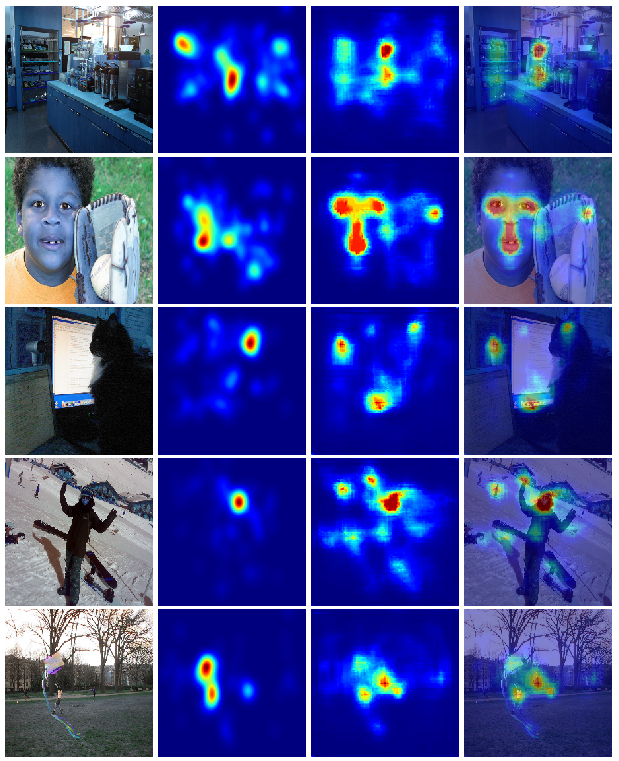
\includegraphics[scale=0.6]{vgg16_predictions_nontrainable.png}
		\caption[Porovnanie predikcií autoenkóderu s VGG16 sieťou bez dodatočného trénovania voči reálnym mapám výraznosti]{
			Porovnanie predikcií autoenkóderu s VGG16 sieťou bez zapnutého učenia, zľava vstupný obrázok, potom originálna mapa výraznosti, predikovaná mapa výraznosti a nakoniec predikcia zobrazená na obrázku.
		}\label{vgg16_predictions_nontrainable}
	\end{center}
\end{figure}

Ako je vidieť na obrázku \ref{vgg16_predictions_nontrainable}, v predikovaných mapách s vypnutým učením na vrstvách VGG16 siete cítiť vplyv detekcie objektov. Sieť vedela relatívne dobre odhadnúť salientné miesta v prípade, že na obrázku nebolo príliš veľa objektov. Problém je ale v intenzite týchto označených miest (tá býva vyššia ako v originálnych mapách) a v situáciách, kedy je na obrázku väčšie množstvo objektov. Vtedy sú v predikovanej mape vizuálnej pozornosti  označené za salientné  aj objekty, ktoré reálne nie sú (napríklad osoby v pozadí, atď.)

\begin{figure}[H]
	\begin{center}
		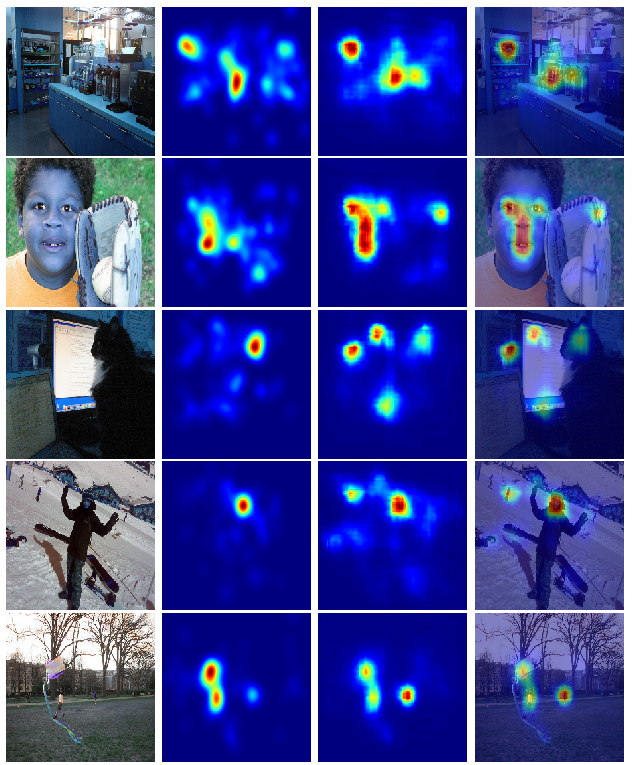
\includegraphics[scale=0.6]{vgg16_predictions_trainable.png}
		\caption[Porovnanie predikcií autoenkóderu s VGG16 sieťou s dodatočným trénovaním voči reálnym mapám výraznosti]{
			Porovnanie predikcií autoenkóderu s VGG16 sieťou so zapnutým učením, zľava vstupný obrázok, potom originálna mapa výraznosti, predikovaná mapa výraznosti a nakoniec predikcia zobrazená na obrázku.
		}\label{vgg_predictions_trainable}
	\end{center}
\end{figure}

Pri zapnutí učenia na vrstvách pre detekciu objektov sa predikcie o niečo zlepšili, sieť pri väčšom počte objektov v scéne už neoznačila tak veľké množstvo za salientné, pri čom aj predikcia intenzity v mapách je miernejšia a viac sa blíži reálnym mapám vizuálnej pozornosti. Zlepšenie koniec koncov potvrdzujú aj metriky vizuálnej pozornosti (popísané v kapitole \ref{metric}), ktorými sme ohodnotili obe konfigurácie modelu. Výsledky sú v tabuľke \ref{vgg16_trainable_vs_nontrainable_metrics}.

\begin{table}[H]
	%\begin{minipage}{\textwidth}
	\centering
	\caption[Porovnanie konfigurácií autoenkóderu s VGG16 sieťou pomocou metrík]{Porovnanie hodnôt metrík pre obe testované konfigurácie}
	\label{vgg16_trainable_vs_nontrainable_metrics}
	\begin{tabular}{{ | p{2cm} |  p{3cm} |  p{3cm} |  p{3cm} |  }}
		\hline
		& \textbf{Model s vypnutým učením pre VGG16 sieť} &  \textbf{Model so zapnutím učením pre VGG16 sieť} \\ \hline
		CC & 0.6863 & 0.8065  \\ \hline
		SIM & 0.6043 & 0.6958  \\ \hline
		AUC & 0.7678 & 0.7832  \\ \hline
		sAUC & 0.7154 & 0.7227 \\ \hline
		NSS & 1.1630 & 1.2381  \\ \hline
	\end{tabular}
	
\end{table}

\subsection{Vedená a upravená vizuálna pozornosť pri modeloch na detekciu objektov}

Ako sme popisovali v kapitole \ref{relu_and_guided_saliency}, pri natrénovaných modeloch k detekcii objektov vieme pár jednoduchými zmenami docieliť, aby sme z nich dostali salientné mapy. V rámci jedného experimentu experimentu sme teda zobrali natrénovanú VGG16 sieť, zmenili sme \textit{softmax} aktivačnú funkciu na lineárnu a postupne použili obe popísané úpravy algoritmu spätného šírenia chyby. Vizualizácie predikcií sú zobrazené na obrázkoch \ref{relu_saliency_predictions} (pre upravenú vizuálnu pozornosť) a \ref{guided_saliency_predictions} (pre vedenú vizuálnu pozornosť). 

\begin{figure}[H]
	\begin{center}
		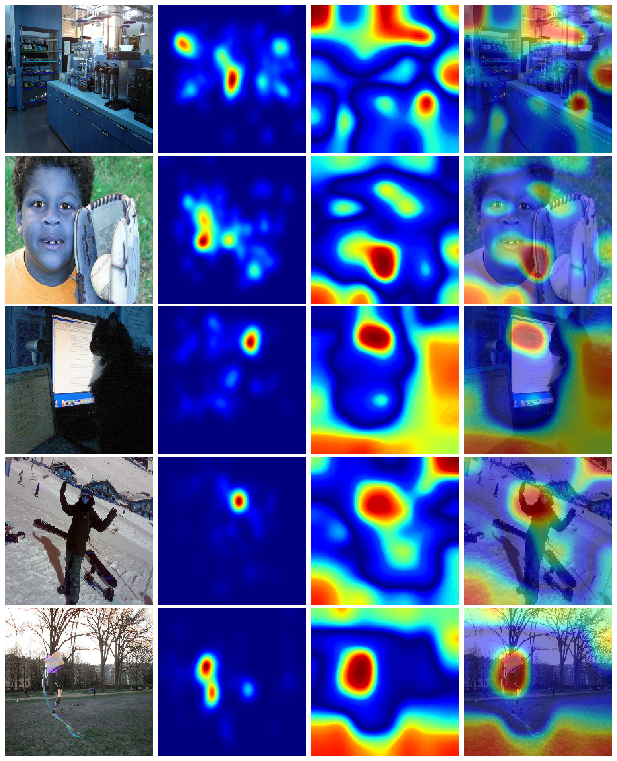
\includegraphics[scale=0.6]{relu_saliency_predictions.png}
		\caption[Porovnanie predikcií upravenej vizuálnej pozornosti voči reálnym mapám výraznosti]{
			Predikcie upravenej vizuálnej pozornosti, zľava vstupný obrázok, potom originálna mapa výraznosti, predikovaná mapa výraznosti a nakoniec predikcia zobrazená na obrázku.
		}\label{relu_saliency_predictions}
	\end{center}
\end{figure}

Vyššie zobrazené vizualizácie ukazujú, že v niektorých prípadoch sa predikcia dokázala zhruba trafiť do salientných miest, tie sú však oveľa rozsiahlejšie ako v originálnych mapách a celkovo majú predikované mapy dosť nízku granularitu. 

\begin{figure}[H]
	\begin{center}
		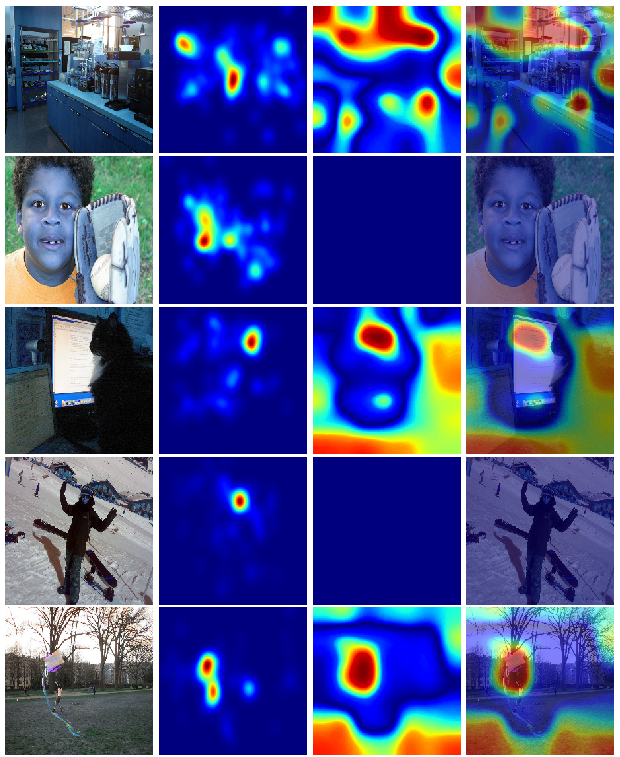
\includegraphics[scale=0.6]{guided_saliency_predictions.png}
		\caption[Porovnanie predikcií vedenej vizuálnej pozornosti voči reálnym mapám výraznosti]{
			Predikcie vedenej vizuálnej pozornosti, zľava vstupný obrázok, potom originálna mapa výraznosti, predikovaná mapa výraznosti a nakoniec predikcia zobrazená na obrázku.
		}\label{guided_saliency_predictions}
	\end{center}
\end{figure}

Pri vedenej vizuálnej pozornosti v zásade pretrvávajú podobné problémy, navyše sa však dosť často stávalo, že sme z modelu neboli schopní dostať žiadne mapy vizuálnej pozornosti. To môže súvisieť s tým, že po úprave algoritmu spätného šírenia chyby sa propaguje iba pozitívny gradient zodpovedný za pozitívne aktivácie. Celkovo predikcie nie sú veľmi presné, presnejšie ale boli mapy práve prvého typu, čo dokázali aj hodnoty metrík vizuálnej pozornosti (kapitola \ref{metric}). Ako je vidieť v tabuľke \ref{relu_vs_guided}, hodnoty metrík nedosahujú veľké čísla, rozdiely medzi dvomi typmi predikcií nie sú až tak veľké.


\begin{table}[H]
	%\begin{minipage}{\textwidth}
	\centering
	\caption[Porovnanie vedenej a upravenej vizuálnej pozornosti]{Porovnanie hodnôt metrík pre predikcie vedenej a upravnej vizuálnej pozornosti}
	\label{relu_vs_guided}
	\begin{tabular}{{ | p{2cm} |  p{3cm} |  p{3cm} |  p{3cm} |  }}
		\hline
		& \textbf{Predikcie vedenej vizuálnej pozornosti (z angl. guided saliency)} &  \textbf{Predikcie upravenej vizuálnej pozornosti (z angl. rectified saliency)} \\ \hline
		CC & 0.0259 & 0.0707  \\ \hline
		SIM & 0.2805 & 0.3040  \\ \hline
		AUC & 0.4973 & 0.5183  \\ \hline
		sAUC & 0.5018 & 0.5155 \\ \hline
		NSS & 0.0204 & 0.0763  \\ \hline
	\end{tabular}
	
\end{table}


\subsection{Porovnanie výsledkov experimentov}
\label{results}

Do výsledného porovnania sme nakoniec zobrali iba modely s najlepšími výsledkami, pri porovnaní sme sa riadili najmä metrikami vizuálnej pozornosti, prehľadné zhrnutie ich hodnôt spolu s chybou na testovacích dátach a veľkosťou vstupných obrázkov je v tabuľke \ref{cnn_vs_autoencoder}

\begin{table}[H]

	\centering
	\caption[Porovnanie konvolučnej neurónovej siete a autoenkóderu]{Porovnanie konvolučnej neurónovej siete a autoenkóderu spolu s hodnotami metrík vizuálnej pozornosti}
	\label{cnn_vs_autoencoder}
	\begin{tabular}{{ | p{1.5cm} |  p{2.5cm} |  p{2.5cm} |  p{2.5cm} | p{2.5cm} | }}
		\hline
		& \textbf{Konvolučná neurónová sieť} &  \textbf{Autoenkóder}  &  \textbf{Kombinácia autoenkóderu s VGG16 sieťou} &  \textbf{Upravená vizuálna pozornosť} \\ \hline
		Veľkosť vstupných obrázkov & 64x64 & 256x256 & 224x224 & 224x224 \\ \hline
		Chyba na testovacích dátach & 0.1459 & 0.01301  & 0.1391 & - \\ \hline
		\textbf{Metriky} &  &  &  &  \\ \hline
		CC & 0.3891 & 0.4634 & 0.8065 & 0.0707\\ \hline
		SIM &  0.3058 & 0.3989 & 0.6958 & 0.3040\\ \hline
		AUC & 0.6892 & 0.7767 & 0.7832 & 0.5183\\ \hline
		sAUC & 0.6631 & 0.7245 & 0.7227 & 0.5155\\ \hline
		NSS & 0.7334 & 1.1288  & 1.2381 & 0.0763\\ \hline
	\end{tabular}
	
	%\end{minipage}
\end{table}

Z vyššie uvedenej tabuľky jasne vyplýva, že najlepšie výsledky má autoenkóder, resp. jeho kombinácia s VGG16 sieťou. I keď hodnoty AUC majú dosť podobné, korelačný koeficient (CC) a podobnosť (SIM), ktoré validujú predikované mapy voči reálnym, nie voči fixáciám, sú výrazne vyššie. Preto sme sa ho rozhodli ako najlepší model, ktorý sa nám podarilo vytvoriť, ďalej porovnať s už existujúcimi modelmi na viacerých datasetoch.

\section{Porovanie najlepšieho modelu s existujúcimi}
%TODO Porovanie najlepšieho modelu s existujúcimi

\iffalse
cnn:

final correlation coeficient: 0.3891757367163311
final SIM: 0.30586936122666497
final NSS: 1.2774279939809017
final judd AUC: 0.8380535277085104
final shuffled AUC: 0.8247464580221275
final borji AUC: 0.8247464580221275

autoencoder:

final correlation coeficient: 0.46347693013377667
final SIM: 0.39894061994859475
final NSS: 1.1588045041398367
final judd AUC: 0.7967435191207479
final shuffled AUC: 0.7245778882530994
final borji AUC: 0.7245778882530994


\fi
